%% -*- coding: utf-8 -*-
\documentclass[12pt,a4paper]{scrartcl} 
\usepackage[utf8]{inputenc}
\usepackage[english,russian]{babel}
\usepackage{indentfirst}
\usepackage{misccorr}
\usepackage{graphicx}
\usepackage{amsmath}
\usepackage{float}

\usepackage{xcolor}
\usepackage{hyperref}
\hypersetup{colorlinks,
  pdftitle={The title of your document},
  pdfauthor={Your name},
  allcolors=[RGB]{000 000 000}}

\begin{document}
\begin{titlepage}
  \begin{center}

    Санкт-Петербургский политехнический университет Петра Великого

    \vspace{0.25cm}
    
    Институт прикладной математики и механики
    
    Кафедра «Прикладная математика»
    \vfill

	\vspace{0.25cm}
	    Отчёт\\
	по курсовой работе\\
	по дисциплине\\
	«Математическая статистика»

  \bigskip

\end{center}
\vfill

\newlength{\ML}
\settowidth{\ML}{«\underline{\hspace{0.7cm}}» \underline{\hspace{2cm}}}
\hfill\begin{minipage}{0.4\textwidth}
  Выполнил студент\\ В.\,А.~Рыженко\\
\end{minipage}%
\bigskip

\hfill\begin{minipage}{0.4\textwidth}
  Проверил:\\
к.ф.-м.н., доцент\\
Баженов Александр Николаевич\\
\end{minipage}%
\vfill

\begin{center}
  Санкт-Петербург, 2020 г.
\end{center}
\end{titlepage}

\tableofcontents
\listoffigures
\newpage

\section{Постановка задачи}
 
Имеется скрипт реализующий функцию интенсивности $I(x, y)$ при заданных параметрах k и NR, где k передаточное числа, а NR количество оборотов вращения солнца вокруг своей оси.
Необходимо написать скрипт в среде Matlab, для поиска таких параметров $k$ и $NR$ из заданного множества, для которых функция $I(x, y)$ имела бы минимальное значение неоднородности по толщине.
Для оптимальных параметров построить график функции дисперсий функций $I(x, y)$, а также графики зависимости толщины напыления вдоль осей.

\section {Реализация}

В качестве критерия минимального значения неоднородности по толщине, было минимальная дисперсия значений функции $I(x, y)$.
Для поиска бы использован был следующий алгоритм.

Вычислялась дисперсия для всех функций $I(x, y)$ на множестве $k\times NR$. Из полученного множества значений дисперсий бралось минимальное и соответствующие ей параметры. Для заданных параметров строилась функция интенсивности напыления.


Все графики были построены при помощи встроенных средств Matlab.
\section{Результаты}
Поиск осуществлялся среди параметров $k = [6, 15, 25, 40, 55]$ и $NR = [12, 18, 24, 28, 35]$.

\begin{figure}[H]
    \centering
    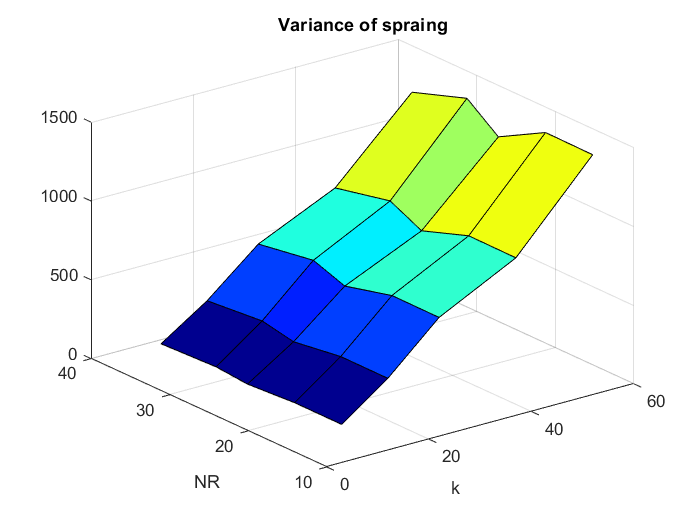
\includegraphics[width=0.6\textwidth]{1.png}
    \caption{График дисперсии значений функции интенсивности напыления}
    \label{fig:f100}
\end{figure}
\begin{figure}[H]
    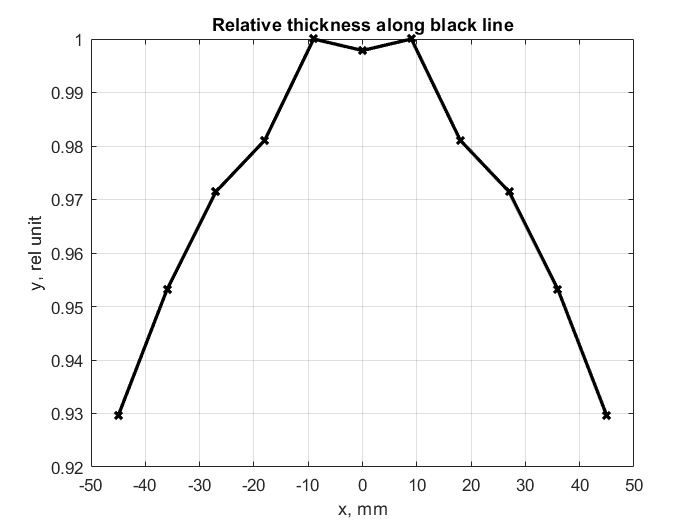
\includegraphics[width=0.6\textwidth]{2.png}
    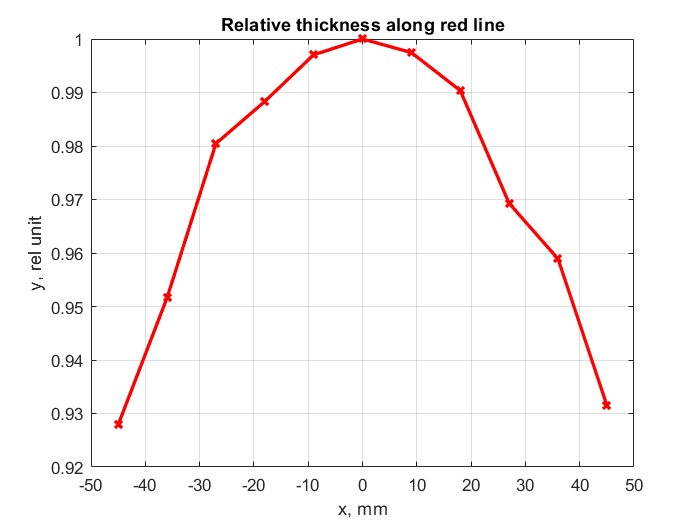
\includegraphics[width=0.6\textwidth]{3.png}
    \caption{Интенсивность напыления вдоль осей при оптимальных параметрах}
    \label{fig:f100}
\end{figure}

Оптимальное значение равномерности напыления получаем при $k = 25$ и $NR = 12$.

\section{Использование}
Для использования программы необходимо задать множество проверяемых параметров $k$ и $NR$. Для это нужно в блоке INPUTS инициализировать переменные k\_input и NR\_input массивам значений соответсвующие проверяемым параметрам.

\section{Приложения}
Репозиторий на GitHub с релизацией: \href{https://github.com/WiillyWonka/MatStat}{github.com}.

\end{document}